\section{実験概要}
本研究で作成したドキュメントの有効性を確認するため, 津田沼チャレンジ\cite{tsudachare}のコースを用いて自律移動実験を行った. 
実験では, ドキュメントによる手順通りにナビゲーションのパラメータを調整されたロボットが, 自律的に設定されたコースを完走できるかで, ドキュメントの妥当性を確認することを目的とした. 

実験は, ドキュメント作成者が2025年度版コースで行ったものと, ROS初心者の学部3年生がドキュメントを参照して2024年度版コースで行ったものの2種類である. 
それぞれのコースを\figref{Fig:Course map of the Tsudanuma Challenge 2025}, \figref{Fig:Course map of the Tsudanuma Challenge 2024}に示す.
ドキュメント作成者を対象とした実験では, 走行地図の作成から自己位置推定および経路計画に関する各種パラメータの調整までを全て行った. 
一方, 学部3年生を対象とした実験では, 作成者がまとめたドキュメントを基に, 作成者が作成した地図を使用してナビゲーションのパラメータ調整を行った. 
また, パラメータ調整に要した時間についても記録し, 調整の負担を把握する参考とした. 

実験には, 本研究室で開発されているロボットORNE-box2\cite{井口颯人2023屋外自律移動ロボットプラットフォーム-orne}を使用した. 
その外観を\figref{Fig:ORNE-box2}に示す. 
また, ナビゲーションにはROS Navigation stackを用いた. 
\begin{figure}[hbtp]
  \centering
 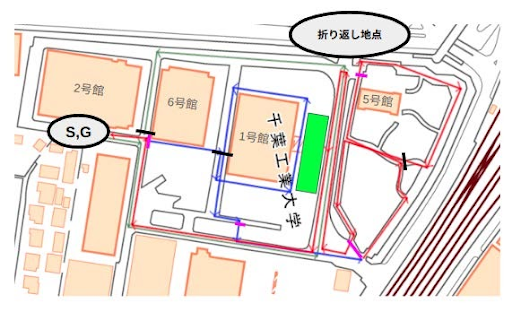
\includegraphics[keepaspectratio, scale=0.5]
      {images/2025tsudacha.png}
 \caption{Course map of the Tsudanuma Challenge 2025(souce: \cite{tsudachare})}
 \label{Fig:Course map of the Tsudanuma Challenge 2025}
\end{figure}
\begin{figure}[hbtp]
  \centering
 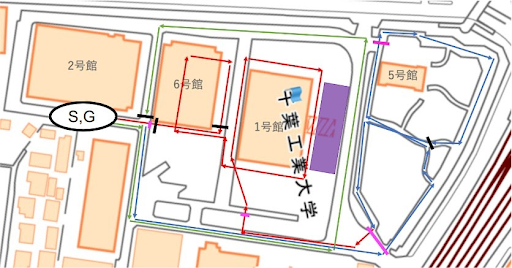
\includegraphics[keepaspectratio, scale=0.5]
      {images/2024tsudacha.png}
 \caption{Course map of the Tsudanuma Challenge 2024(souce: \cite{tsudachare})}
 \label{Fig:Course map of the Tsudanuma Challenge 2024}
\end{figure}
\begin{figure}[hbtp]
  \centering
 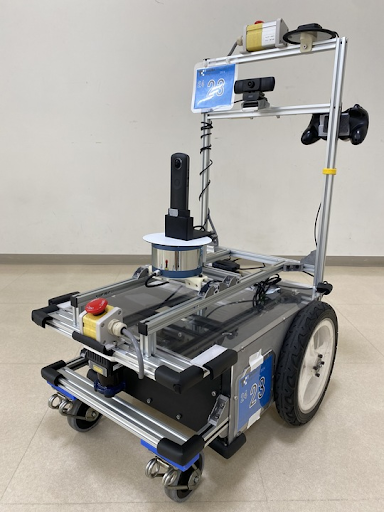
\includegraphics[keepaspectratio, scale=0.3]
      {images/box2.png}
 \caption{ORNE-box2}
 \label{Fig:ORNE-box2}
\end{figure}




\newpage
\section{実験結果}
\subsection{ドキュメント作成者が行った実験結果}
\begin{table}[htbp]
  \centering
  \caption{Navigation results of the Tsudanuma Challenge 2025}
  \label{tab:tsudanuma_result}
  \begin{tabular}{lcc}
    \hline
    \textbf{Run type} & \textbf{Number of trials} & \textbf{Number of success} \\
    \hline
    Preliminary run & 10 & 10 \\
    Official run        & 1  & 1  \\
    \hline
  \end{tabular}
\end{table}
\tabref{tab:tsudanuma_result}に示すように, 調整後のシステムを用いて事前走行を10回実施した結果, すべての試行でゴールまでの完走を確認した. 
さらに,本走行においてもコースを完走し, 自己位置の破綻や経路追従の失敗は見られなかった. 

\subsection{学部3年生が行った実験結果}
\begin{table}[htbp]
  \centering
  \caption{Results of B3 students in the Tsudanuma Challenge 2024}
  \label{tab:b3_results}
  \begin{tabular}{lccc}
    \hline
     & \textbf{No.1} & \textbf{No.2} & \textbf{No.3} \\
    \hline
    Completion & Yes & Yes & Yes \\
    Total time to completion [h] & 5.0 & 3.5 & 4.5 \\
    \hline
  \end{tabular}
\end{table}
\tabref{tab:b3_results}に示すように, ドキュメントの手順に沿ってパラメータ調整を行った結果, 3名ともコースの完走を達成することができた. 
いずれの実験においても, ロボットは経路から大きく逸脱することなく目標地点まで走行でき, 安定したナビゲーション動作が確認された. 
また, パラメータ調整に要した時間は3.5〜5.0時間であり, いずれの参加者も作業を完遂することができた. 
これにより,ドキュメントの妥当性が一定程度担保されていることが確認された. 


